%
% anwendungen.tex -- Anwendungen der elliptischen Funktionen
%
% (c) 2026 Baris Catan, OST Ostschweizer Fachhochschule
%
% !TEX root = ../../buch.tex
% !TEX encoding = UTF-8
%
\section{Anwendungen
\label{elliptisch:section:anwendungen}}
\kopfrechts{Anwendungen}

Mit dem Werkzeugkasten von
Abschnitt~\ref{elliptisch:subsection:werkzeugkasten} ist klar, woran
man eine jacobische Lösung erkennt.
Führt ein Problem auf die Differentialgleichung
\eqref{elliptisch:equation:signatur}, also das Quadrat der Ableitung
gleich einem Polynom vierten Grades, dann ist die Lösung eine
jacobische Funktion.
In diesem Abschnitt taucht diese Signatur dreimal auf.
Wir beginnen bei der Kurve, an der die Theorie historisch ihren
Anfang genommen hat, und kommen danach zu zwei physikalischen
Problemen, einem rotierenden Seil und einem Pendel.

\subsection{Die Lemniskate
\label{elliptisch:subsection:lemniskate}}
\index{Lemniskate}%
Die \emph{Lemniskate von Bernoulli} ist die Kurve vierten Grades
mit der Gleichung
\begin{equation}
(X^2+Y^2)^2 = 2a^2\,(X^2-Y^2).
\label{elliptisch:equation:lemniskate}
\end{equation}
Wir verwenden die Normierung $a = 1/\sqrt{2}$, in der die Scheitel
bei $(\pm 1, 0)$ liegen (Abbildung~\ref{fig:elliptisch:lemniskate}).
\begin{figure}
	\centering
	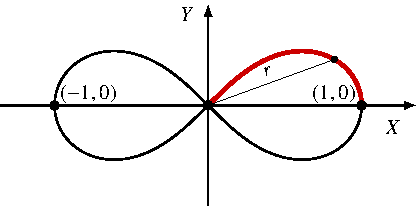
\includegraphics[width=0.56\textwidth]{papers/elliptisch/images/lemniskate.pdf}
	\caption{Die Lemniskate von Bernoulli mit $a = 1/\sqrt{2}$ und
	den Scheiteln bei $(\pm 1, 0)$.
	Hervorgehoben ist der Bogen vom Nullpunkt bis zum Scheitel
	$(1,0)$, seine Länge ist $\varpi/2$.}
	\label{fig:elliptisch:lemniskate}
\end{figure}
%
In Polarkoordinaten schreibt sie sich als $r^2 = \cos 2\varphi$.
Das Bogenelement in Polarkoordinaten ist
$ds^2 = dr^2 + r^2\,d\varphi^2$ und Differenzieren der
Kurvengleichung ergibt $2r\,dr = -2\sin 2\varphi\,d\varphi$.
Damit lässt sich $\varphi$ eliminieren,
\begin{equation}
r^2\,d\varphi^2
=
\frac{r^4}{\sin^2 2\varphi}\,dr^2
=
\frac{r^4}{1-r^4}\,dr^2,
\label{elliptisch:equation:phielimination}
\end{equation}
denn es ist $\sin^2 2\varphi = 1 - \cos^2 2\varphi = 1 - r^4$.
Somit bleibt im Bogenelement nur noch der Radius,
\begin{equation}
ds
=
\sqrt{1 + \frac{r^4}{1-r^4}}\,dr
=
\frac{dr}{\sqrt{1-r^4}}.
\label{elliptisch:equation:bogenelementr}
\end{equation}
Die Bogenlänge vom Nullpunkt bis zum Punkt mit Radius $r$ ist damit
\begin{equation}
s(r)
=
\int_0^r \frac{dt}{\sqrt{1-t^4}}.
\label{elliptisch:equation:lemniskatebogen}
\end{equation}
Unter der Wurzel steht mit $1-t^4 = (1-t^2)(1+t^2)$ wieder ein
Polynom vierten Grades ohne mehrfache Nullstellen, das Integral
fällt also unter die Definition
\eqref{elliptisch:equation:definition}.
Der direkte Vergleich mit der Normalform
\eqref{elliptisch:equation:normalformen} liefert formal
$k^2 = -1$, ausserhalb des Bereichs von
Satz~\ref{elliptisch:satz:nichtelementar}.
Wie Gleichung \eqref{elliptisch:equation:sljacobi} weiter unten
zeigt, gehört das Integral nach einer Substitution zum Modul
$k = 1/\sqrt{2}$, und weil diese Substitution algebraisch ist,
überträgt sich der Satz, eine elementare Stammfunktion existiert
nicht.
Der Kontrast zum Kreis wiederholt sich.
Das Integral $\int_0^r dt/\sqrt{1-t^2} = \arcsin r$ bleibt
elementar, das Bogenlängenintegral der Lemniskate nicht.

Wie in \eqref{elliptisch:equation:umkehrung} kehren wir um.
Die Umkehrfunktion $r = \operatorname{sl}(s)$ heisst
\emph{lemniskatischer Sinus}.
\index{lemniskatischer Sinus}%
Leitet man \eqref{elliptisch:equation:lemniskatebogen} nach $s$ ab,
folgt $(\operatorname{sl}')^2 = 1 - \operatorname{sl}^4$, wieder die
Signatur \eqref{elliptisch:equation:signatur} aus dem
Werkzeugkasten.
Der Bogen vom Nullpunkt bis zum Scheitel $(1,0)$ hat die Länge
$\varpi/2$, wobei
\begin{equation}
\varpi
=
2\int_0^1 \frac{dt}{\sqrt{1-t^4}}
=
2.6220575542\ldots
\label{elliptisch:equation:varpi}
\end{equation}
die Länge des rechten Blattes ist, die sogenannte
\emph{lemniskatische Konstante}.
\index{lemniskatische Konstante}%
Die Funktion $\operatorname{sl}$ ist $2\varpi$-periodisch, und was
für den Sinus die Zahl $\pi$ ist, ist für ihn $\varpi$.
Historisch war der lemniskatische Sinus die erste elliptische
Funktion überhaupt.
Gauss hat sie 1797 als Neunzehnjähriger in seinem mathematischen
Tagebuch untersucht, zu Lebzeiten aber nichts davon veröffentlicht
\cite{elliptisch:almkvist-berndt} und
\cite[Abschnitt~11.3]{elliptisch:mueller-spezielle}.
Erst dreissig Jahre später wurde derselbe Umkehrschritt von Abel
und Jacobi in voller Allgemeinheit vollzogen
(Abschnitt~\ref{elliptisch:subsection:unvollstaendig}).

Die Verbindung zu den jacobischen Funktionen gewinnt man aus der
Bogenlängenparametrisierung der Lemniskate.
Aus ihr folgt
\begin{equation}
\operatorname{sl}(s)
=
\operatorname{cn}\biggl(
\sqrt{2}\,\Bigl(\frac{\varpi}{2}-s\Bigr),\,
\frac{1}{\sqrt{2}}
\biggr),
\label{elliptisch:equation:sljacobi}
\end{equation}
der lemniskatische Sinus ist also bis auf Skalierung und
Verschiebung des Arguments die Funktion $\operatorname{cn}$ zum
Modul $k = 1/\sqrt{2}$
\cite[Abschnitt~11.3]{elliptisch:mueller-spezielle}.
Insbesondere ist $\varpi = \sqrt{2}\,K(1/\sqrt{2})$, ganz analog zu
$\pi = 2K(0)$ in \eqref{elliptisch:equation:randnull}.

\subsection{Das Troposkein
\label{elliptisch:subsection:troposkein}}
\index{Troposkein}%
\index{Springseil}%
Eine Schnur hängt zwischen zwei Punkten $A$ und $B$.
Unter der Schwerkraft nimmt sie die Kettenlinie an, einen
hyperbolischen Kosinus, ein durch und durch elementares Resultat.
Lassen wir dieselbe Schnur stattdessen mit der
Winkelgeschwindigkeit $\omega$ um die Verbindungsachse von $A$
und $B$ rotieren und vernachlässigen die Schwerkraft, entsteht
eine neue Gleichgewichtsform.
Sie heisst \emph{Troposkein} oder Springseilkurve
\cite{elliptisch:skipping-rope}.
Abbildung~\ref{fig:elliptisch:troposkein} zeigt das Profil der
rotierenden Schnur zwischen $A$ und $B$.
\begin{figure}
	\centering
	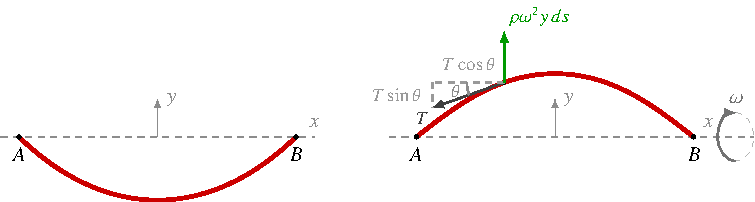
\includegraphics[width=\textwidth]{papers/elliptisch/images/troposkein.pdf}
	\caption{Links die hängende Schnur zwischen $A$ und $B$ bei
	$x = \pm l$, die Kettenlinie
	$y(x) = d\,(\cosh(x/d) - \cosh(l/d))$.
	Rechts rotierend um $AB$, das Troposkein
	\mbox{$y(x) = a\operatorname{sn}((x+l)/c, k)$}, mit
	Zentrifugalkraft $\rho\omega^2y\,ds$ und Seilspannung $T$ am
	Element mit Winkel $\theta$.}
	\label{fig:elliptisch:troposkein}
\end{figure}
%

Wir bezeichnen mit $y(x)$ den Abstand eines Seilpunktes von der
Drehachse, mit $\theta$ den Winkel der Seiltangente gegen die
Achse, mit $\rho$ die Linienmassendichte und mit $T$ die
Seilspannung (Abbildung~\ref{fig:elliptisch:troposkein}, rechts).
Auf ein Element der Länge $ds$ wirkt die Zentrifugalkraft
$\rho\omega^2 y\,ds$ radial nach aussen.
Im Gleichgewicht ist die axiale Komponente der Spannung konstant,
\begin{equation}
T\cos\theta = T_0,
\label{elliptisch:equation:troposkeinaxial}
\end{equation}
und die Änderung ihrer Querkomponente entlang der Bogenlänge trägt
die Zentrifugalkraft,
\begin{equation}
\frac{d(T\sin\theta)}{ds}
=
-\rho\omega^2 y.
\label{elliptisch:equation:troposkeinradial}
\end{equation}
Aus \eqref{elliptisch:equation:troposkeinaxial} folgt durch
Differenzieren die Beziehung
$dT/ds = \sin\theta \cdot d(T\sin\theta)/ds$.
Multipliziert man \eqref{elliptisch:equation:troposkeinradial} mit
$\sin\theta$, steht damit
\begin{equation}
\frac{dT}{ds}
=
-\rho\omega^2 y\,\frac{dy}{ds},
\label{elliptisch:equation:troposkeinintegration}
\end{equation}
und die Integration nach $y$ liefert
die Spannung als Funktion des Abstandes,
\begin{equation}
T(y)
=
T_0 + \frac{\rho\omega^2}{2}\,\bigl(a^2 - y^2\bigr),
\label{elliptisch:equation:troposkeinspannung}
\end{equation}
wobei $a$ der grösste Achsabstand ist, also der Scheitel der Kurve,
an dem $\theta = 0$ und $T = T_0$ gilt.
Die Spannung ist folglich in der Mitte am kleinsten und an den
Endpunkten am grössten.

Die Ableitung der Kurve ist $y' = \tan\theta$, und mit
$\tan^2\theta = (T/T_0)^2 - 1$ wird aus
\eqref{elliptisch:equation:troposkeinspannung} nach Quadrieren und
Zusammenfassen der Konstanten
\begin{equation}
(y')^2
=
\frac{1}{c^2}\,\bigl(a^2 - y^2\bigr)
\biggl(1 - \frac{b^2 y^2}{a^4}\biggr)
\label{elliptisch:equation:troposkein}
\end{equation}
mit zwei Konstanten $b \le a$ und $c$, die sich aus den
physikalischen Grössen und den Randbedingungen bestimmen.
Rechts steht ein Polynom vierten Grades in $y$, genau die Signatur
\eqref{elliptisch:equation:signatur} aus dem Werkzeugkasten.
Die Lösung muss daher eine jacobische Funktion sein.
Wir machen den Ansatz, mit $x$ von der Mitte aus gemessen und
$A$ bei $x = -l$,
\begin{equation}
y(x)
=
a\,\operatorname{sn}\Bigl(\frac{x+l}{c}, k\Bigr),
\qquad
k = \frac{b}{a},
\label{elliptisch:equation:troposkeinloesung}
\end{equation}
und setzen ihn zur Probe ein.
Nach \eqref{elliptisch:equation:sndgl} ist
$(y')^2 = (a^2/c^2)\,\operatorname{cn}^2\operatorname{dn}^2
= (1/c^2)\,(a^2-y^2)\,(1 - k^2y^2/a^2)$,
was mit $k = b/a$ genau die rechte Seite von
\eqref{elliptisch:equation:troposkein} ergibt.
Die Randbedingungen legen die Konstanten fest.
Das Seil geht bei $A$ und $B$ durch $y = 0$ und erreicht seine
grösste Auslenkung in der Mitte, also ist $l = c\,K(k)$, und die
vorgegebene Seillänge liefert die zweite Bedingung an $b$ und $c$.

Welche Form das Seil annimmt, bestimmt der Modul, und der kommt
aus der Physik.
Setzt man \eqref{elliptisch:equation:troposkeinspannung} in
$(y')^2 = (T/T_0)^2 - 1$ ein und vergleicht mit
\eqref{elliptisch:equation:troposkein}, liest man
\begin{equation}
k^2
=
\frac{b^2}{a^2}
=
\frac{a^2}{a^2 + 4T_0/(\rho\omega^2)}
\label{elliptisch:equation:troposkeinmodul}
\end{equation}
ab.
Schnelle Rotation bei schwacher Spannung treibt $k$ gegen $1$,
starke Spannung gegen $0$.

Damit stellt sich heraus, dass das Auge uns hier täuscht.
Die Springseilkurve sieht aus wie eine Sinushalbwelle, ist aber ein
jacobischer Sinus als Funktion des \emph{Ortes}.
Was die Form verändert, ist allein der Modul.
Nach den Grenzfällen aus
Abschnitt~\ref{elliptisch:subsection:werkzeugkasten} ist
$\operatorname{sn}$ für $k = 0$ der gewöhnliche Sinus, während die
Halbwelle für $k \to 1$ ein Plateau und steile Flanken bekommt.
Mit \eqref{elliptisch:equation:troposkeinmodul} wird dieses Plateau
also breiter, je schneller das Seil rotiert.
Dieselbe Signatur \eqref{elliptisch:equation:signatur} wird uns
in Abschnitt~\ref{elliptisch:subsection:pendel} wieder begegnen,
dort mit der Zeit als unabhängiger Variable.

Die Form hat auch eine technische Seite.
Die Schaufeln des Darrieus-Rotors werden im Troposkein-Profil
gebaut, weil die Zentrifugalkraft ein Seil in dieser Form nur auf
Zug belastet und nicht auf Biegung
\cite{elliptisch:wiki-darrieus}.
\index{Darrieus-Rotor}%
Dessen Achse steht senkrecht, und damit wirkt die Schwerkraft
längs der Achse.
Sie geht in die axiale Bilanz ein, aus
\eqref{elliptisch:equation:troposkeinaxial} wird
$d(T\cos\theta)/ds = \rho g$, und das Troposkein ist nur noch eine
Näherung.
Bei Betriebsdrehzahl ist $\omega^2 y$ jedoch um Grössenordnungen
grösser als $g$, sodass die Abweichung klein bleibt.
\begin{figure}
	\centering
	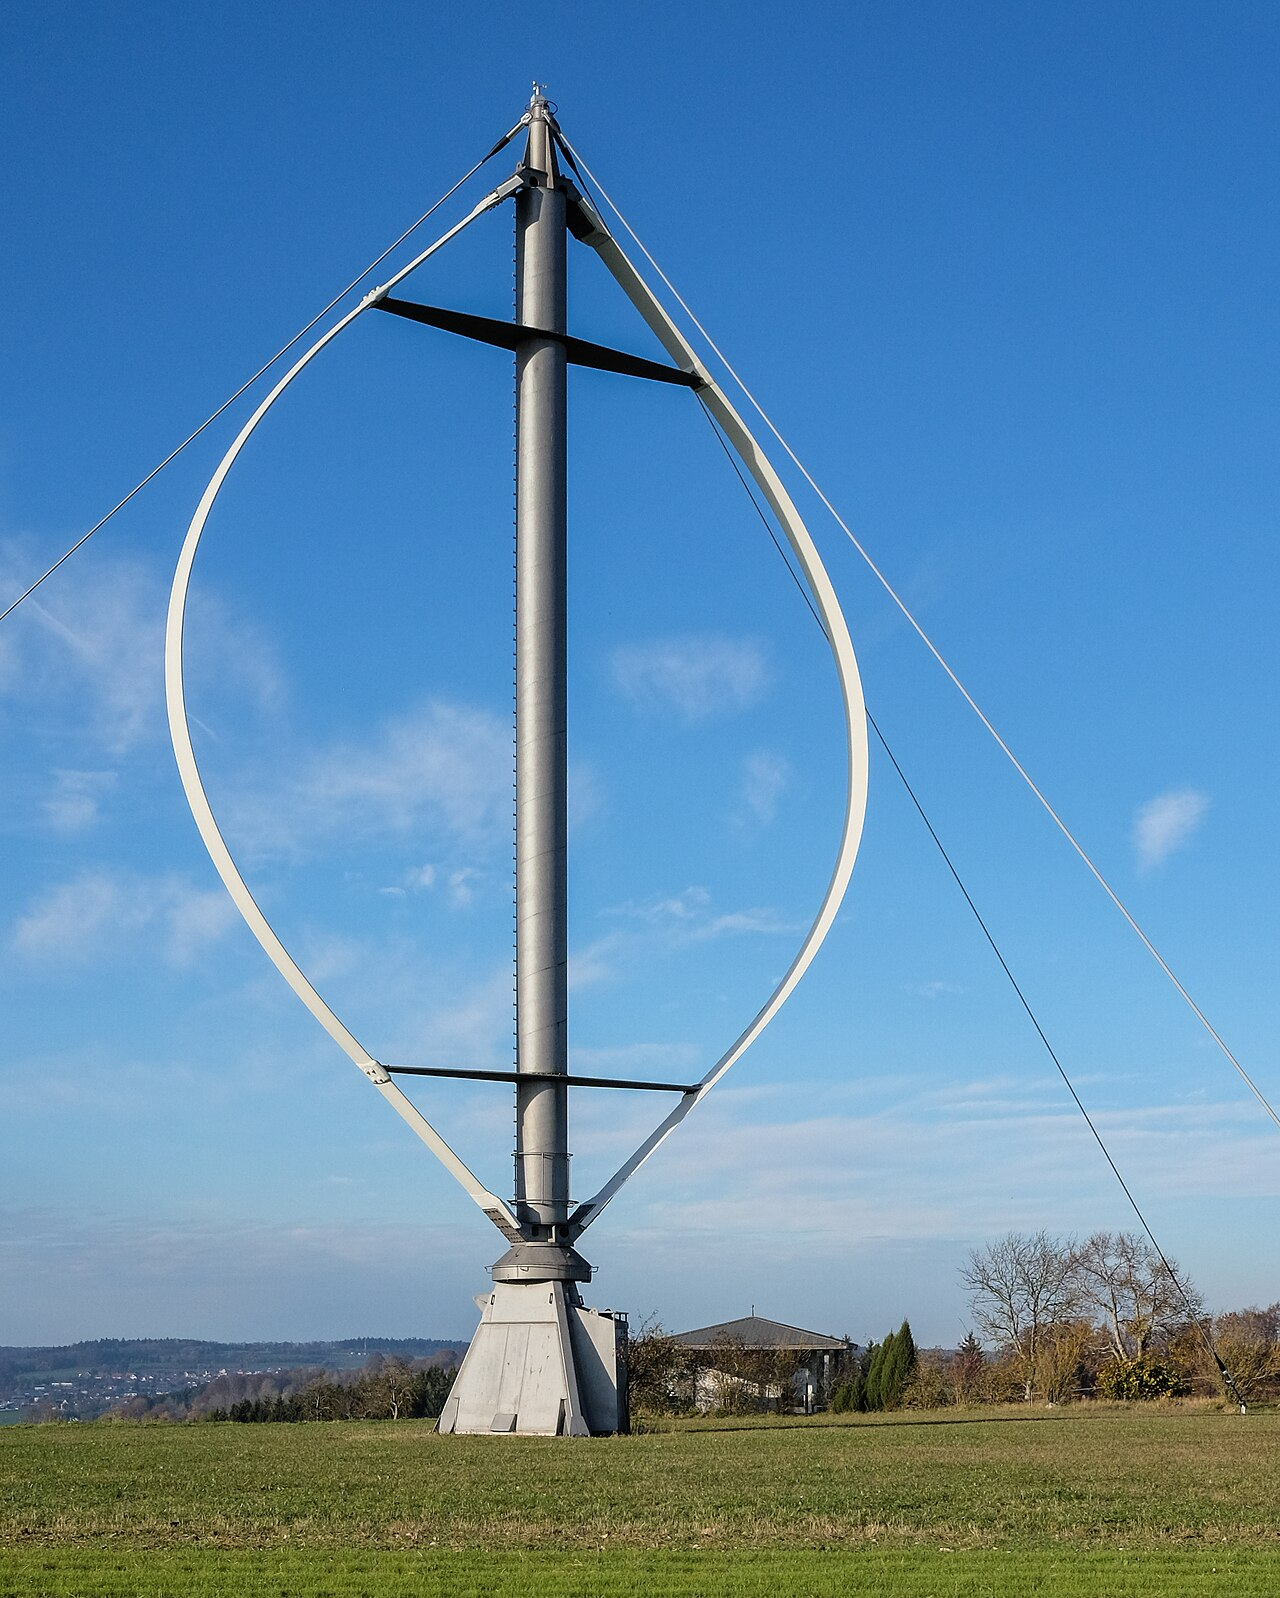
\includegraphics[width=0.5\textwidth]{papers/elliptisch/images/darrieus-rotor.jpg}
	\caption{Ein Darrieus-Rotor mit zwei Schaufeln im
	Troposkein-Profil.
	Bild: \cite{elliptisch:darrieus-bild}.}
	\label{fig:elliptisch:darrieus}
\end{figure}


\subsection{Das Pendel
\label{elliptisch:subsection:pendel}}
Wie am Ende von Abschnitt~\ref{elliptisch:subsection:troposkein}
angekündigt, begegnet uns die Signatur
\eqref{elliptisch:equation:signatur} jetzt mit der Zeit als
unabhängiger Variable.
Ein Massepunkt der Masse $m$ hängt an einem masselosen Stab der
Länge $l$, und $\vartheta$ sei der Auslenkwinkel gegen das Lot
(Abbildung~\ref{fig:elliptisch:pendel}, links).
\begin{figure}
	\centering
	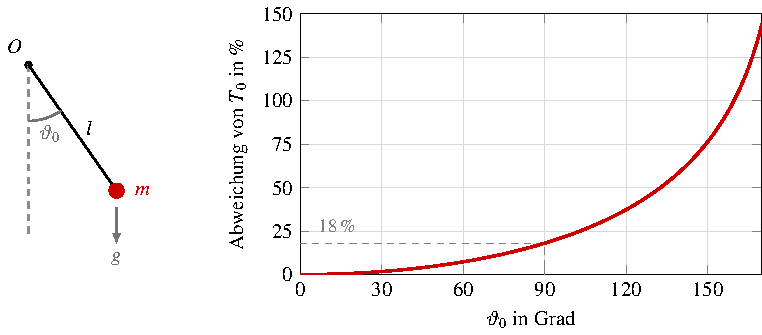
\includegraphics[width=\textwidth]{papers/elliptisch/images/pendel.pdf}
	\caption{Links das mathematische Pendel der Länge $l$ mit der
	Amplitude $\vartheta_0$.
	Rechts die Abweichung der exakten Schwingungsdauer
	$T = 4\sqrt{l/g}\,K(k)$ von der Kleinwinkelnäherung
	$T_0 = 2\pi\sqrt{l/g}$ in Prozent, aufgetragen über
	$\vartheta_0$.
	Bei $90^\circ$ sind es $18\,\%$.}
	\label{fig:elliptisch:pendel}
\end{figure}
%
Die Bewegungsgleichung des Pendels ist
\begin{equation}
\ddot{\vartheta} = -\frac{g}{l}\,\sin\vartheta.
\label{elliptisch:equation:pendelbewegung}
\end{equation}
Wir verzichten auf die Kleinwinkelnäherung
\index{Kleinwinkelnäherung}%
$\sin\vartheta \approx \vartheta$ und rechnen exakt.

Die Multiplikation von \eqref{elliptisch:equation:pendelbewegung}
mit $\dot\vartheta$ und Integration über die Zeit liefert die
Energieerhaltung, ein erstes Integral der Bewegungsgleichung.
Startet das Pendel aus der Ruhe bei der Amplitude $\vartheta_0$, so
ist
\begin{equation}
\frac{1}{2}\,ml^2\dot\vartheta^2 + mgl\,(1-\cos\vartheta)
=
mgl\,(1-\cos\vartheta_0).
\label{elliptisch:equation:pendelenergie}
\end{equation}
Mit $1-\cos\vartheta = 2\sin^2(\vartheta/2)$ folgt
$\dot\vartheta^2 = (4g/l)\,\bigl(\sin^2(\vartheta_0/2)
-\sin^2(\vartheta/2)\bigr)$, und die Substitution
$y = \sin(\vartheta/2)$ mit
$\dot y^2 = \frac14\,(1-y^2)\,\dot\vartheta^2$ ergibt
\begin{equation}
\dot y^2
=
\frac{g}{l}\,(1-y^2)\,\bigl(y_0^2-y^2\bigr),
\qquad
y_0 = \sin\frac{\vartheta_0}{2}.
\label{elliptisch:equation:pendeldgl}
\end{equation}
Rechts steht wieder die Signatur
\eqref{elliptisch:equation:signatur}.
Die Normierung $z = y/y_0$ auf die Amplitude und
$u = \sqrt{g/l}\,t$ auf die Zeit macht daraus
\begin{equation}
\biggl(\frac{dz}{du}\biggr)^2
=
(1-z^2)\,\bigl(1-y_0^2 z^2\bigr),
\label{elliptisch:equation:pendelnormiert}
\end{equation}
exakt die Gleichung \eqref{elliptisch:equation:sndgl} des
jacobischen Sinus.
Damit ist $z = \operatorname{sn}(u,k)$ mit dem Modul
$k = y_0 = \sin(\vartheta_0/2)$, der die Amplitude misst.
Die Energie ist $E = 2mgl\,k^2$
\cite[Abschnitt~11.2.3]{elliptisch:mueller-spezielle}.

Jetzt machen wir die beiden Substitutionen rückgängig.
Aus $z = y/y_0$ und $k = y_0$ wird
$y = y_0 z = k\,\operatorname{sn}(u,k)$, und mit
$y = \sin(\vartheta/2)$ sowie $u = \sqrt{g/l}\,t$ ist
\begin{equation}
\sin\frac{\vartheta}{2}
=
k\,\operatorname{sn}\bigl(\sqrt{g/l}\;t,\,k\bigr),
\qquad\text{also}\qquad
\vartheta(t)
=
2\arcsin\Bigl(k\,\operatorname{sn}\bigl(\sqrt{g/l}\;t,\,k\bigr)\Bigr).
\label{elliptisch:equation:pendelloesung}
\end{equation}
Eine volle Schwingung durchläuft in $u$ die Periode $4K(k)$.
Gesucht ist aber die Periode in der Zeit und nicht in $u$.
Wegen $t = u\sqrt{l/g}$ wird daraus die Schwingungsdauer
\begin{equation}
T = 4\,\sqrt{\frac{l}{g}}\;K(k).
\label{elliptisch:equation:pendelperiode}
\end{equation}

Für kleine Amplituden geht $k$ gegen $0$, und mit $K(0) = \pi/2$
aus \eqref{elliptisch:equation:randnull} kommt
$T \to 2\pi\sqrt{l/g}$ heraus, die Kleinwinkelnäherung kehrt als
Grenzfall zurück.
Bei $\vartheta_0 = 90^\circ$ ist die Periode bereits um $18\,\%$
länger als die Kleinwinkelformel, bei $\vartheta_0 = 179^\circ$
um den Faktor $3.9$
(Abbildung~\ref{fig:elliptisch:pendel}, rechts).
Für $k \to 1$, also $\vartheta_0 \to \pi$, divergiert $K(k)$
logarithmisch wie in \eqref{elliptisch:equation:kasymptotik}, und
die Schwingungsdauer wächst über alle Grenzen, das Pendel erreicht
den oberen Scheitelpunkt asymptotisch nie.
